\documentclass[hyperref={bookmarks=true}, aspectratio=43]{beamer}
\usepackage[utf8]{inputenc}
\usepackage[T1]{fontenc}
\usepackage[ngerman, english]{babel}
\usepackage{booktabs}
\usepackage{multirow}
\hypersetup{bookmarksopen=true,bookmarksopenlevel=3}
\usepackage{verbatim}
\usepackage{microtype}
\usepackage{tikz}
\usetikzlibrary{positioning}
\usetikzlibrary{arrows}
\usetikzlibrary{shadows}

\usepackage{lmodern}
\usepackage{hyperref}
\usepackage[skins]{tcolorbox}
\usepackage{pdfpages}
\usepackage{eurosym}
\usepackage{upgreek}
\usepackage{amsmath}
\usepackage{amssymb}
\usepackage{textcomp}
\usepackage{listings}
\usepackage{multicol}

% Stata Farben
\definecolor{Statafunction}{HTML}{0000FF}
\definecolor{Statacomment}{HTML}{007F00}
\definecolor{Statastring}{HTML}{7F0000}
\definecolor{Statakeywords}{HTML}{00007F}
\definecolor{Statamacro}{HTML}{007F7F}


% Ich weiss nicht, was [b] macht [l = line] [s = string] [b = behind?]
\lstset{
    keywordstyle=\color{Statakeywords}
  , basicstyle=\scriptsize\ttfamily
  , commentstyle=\color{Statacomment}
  , columns=flexible
  , upquote=true
  , comment=[l][\color{Statacomment}]{**}
  , morecomment=[l][\color{Statacomment}]{***}
  , morecomment=[s][\color{Statacomment}]{/*}{*/}
  , morecomment=[l][\color{Statacomment}]{///}
  , morecomment=[l][\color{Statacomment}]{//}
  , morestring=[s][\color{Statastring}]{"}{"}
  , morestring=[s][\color{Statamacro}]{`}{'}
  , showstringspaces=false
  , literate=%
    {Ö}{{\"O}}1
    {Ä}{{\"A}}1
    {Ü}{{\"U}}1
    {ß}{{\ss}}2
    {ü}{{\"u}}1
    {ä}{{\"a}}1
    {ö}{{\"o}}1
  }

% Bei Optionen von Befehlen gibt es ein paar Abweichungen von der Stata 12 Syntax. Da Stata hier aber auch inkonsistent
% ist, ignoriere ich das fürs erste.
% Bswp: tab var1, sum(var2) soll // sum hellblau sein.
%       tab var1, summarize(var2) // soll summarize keine Farbe haben.
%       tab var1, by(var2) // soll by keine Farbe haben
\lstset{emph={%  
    _a_cls_msg, _addgph, _applycoding, _asprobit_diparm, _asprobit_estimator, _asprobit_replay, _asprobit_vce_parserun, _assert, _assert_mreldif, _assert_mreldifp, _assert_mreldifs, _assert_obs, _assert_streq, _at,
    _b_fill0, _b_post0, _bigtab, _binomial2bernoulli, _binperfect, _binperfout, _biplotmat, _biplotmat_10, _brr_sum, _bs_display, _bs_sum, _btcmd, _byoptnotallowed, _ca_process_mlabel, _callerr, _canon, _cci,
    _check4gropts, _check_e_margins, _check_e_rc, _check_eformopt, _check_numeric_vtype, _check_omit, _check_ts_gaps, _checkpd, _ckirfset, _cknotsvaroi, _ckvec, _clsarr2list, _cmdxel, _coef_table, _coef_table_header,
    _confirm_date, _confirm_number_or_date, _copy_mat_stripes, _cpmatnm, _crc2use, _crc4fld, _crcacnt, _crcar1, _crcause, _crcbin, _crcbygr, _crcchi2, _crcchkw, _crccip, _crceprs, _crcgldv, _crcglil, _crcird, _crcirr,
    _crcmeq, _crcnuse, _crcor, _crcphdr, _crcra, _crcrd, _crcrr, _crcseq, _crcshdr, _crcslbl, _crcsrvc, _crcswxx, _crcunab, _crcunit, _crcvarl, _crcwsrv, _crczsku, _cvar, _datasig, _datasign, _datasigna, _datasignat,
    _datasignatu, _datasignatur, _datasignature, _date2elapsed, _diag2mat, _diparm, _diparm_8, _dm_create, _dots, _dvech_estat, _dvech_falast, _e2r, _egennoby, _epitab_by_parse, _ereturn_display, _est, _estat_icc, _esti,
    _estim, _estima, _estimat, _estimate, _estimates, _evlist, _exactreg_coef, _exactreg_lf, _exactreg_p, _exactreg_replay, _exactreg_replayse, _exactreg_sort, _exactreg_tests, _exp_list_expand, _exp_list_parse,
    _favor_parse, _find_tsops, _findhlpalias, _float2binary, _fr_area_parse_and_log, _fr_aspect_parse_and_log, _fr_clegend_parse_and_log, _fr_declare_date_line, _fr_draw_rect, _fr_droplines_draw, _fr_erasearr,
    _fr_legend_parse_and_log, _fr_merged_implicit, _fr_runlog, _fr_sztextbox_parse_and_log, _fr_tbstyle_parse_and_log, _fr_tedits_parse_and_log, _fr_textbox_parse_and_log, _fr_title_parse_and_log, _fr_x_log_cleanup,
    _fr_x_log_create, _fr_zyx2legend_parse_and_log, _fracpp, _fracxo, _frr_sztextbox_pnl, _fv_check_depvar, _gany, _ganycount, _ganymatch, _ganyvalue, _gconcat, _gcount, _gcut, _gdiff, _gends, _geqany, _get_diopts,
    _get_diparmopts, _get_diparmopts_8, _get_eformopts, _get_eqspec, _get_gropts, _get_hmat, _get_irf, _get_mcompare, _get_offopt, _getbv, _getcovcorr, _getfilename, _getmlogitcoef, _getnewlabelname, _getrhs, _getvarcns,
    _getxel, _getxel2, _gfill, _ggroup, _giqr, _gkurt, _gm_dlg_edits, _gm_edit, _gm_log, _gm_logadd_in, _gm_splitlog, _gma, _gmad, _gmax, _gmdev, _gmean, _gmedian, _gmin, _gmode, _gmode10, _gmtr, _gneqany, _gpc, _gpctile,
    _gr_applytrans, _gr_arrowhead, _gr_atomize_styles, _gr_common_axes, _gr_drawrect, _gr_linkstyles, _gr_symbol_of, _grank, _grfirst, _grlast, _grmax, _grmean, _grmin, _grmiss, _grobs, _growfirst, _growlast, _growmax,
    _growmean, _growmedian, _growmin, _growmiss, _grownonmiss, _growpctile, _growsd, _growtotal, _grsd, _grsum, _gs_addgrname, _gs_by_combine, _gs_bygraph, _gs_byopts_combine, _gs_clean_graphlist, _gs_default_bands,
    _gs_islivefile, _gs_parse_and_log_axoptions, _gs_parse_and_log_axtitle, _gs_parse_and_log_lines, _gs_parse_and_log_tickset, _gs_path2memname, _gs_rdfilehdr, _gs_rec_rdfilehdr, _gs_rec_wrfilehdr, _gs_rtmostofclass,
    _gs_wrfilehdr, _gs_x_create, _gsd, _gseq, _gskew, _gstd, _gsum, _gtag, _gtotal, _hadamard_verify, _hw_comp, _hw_opt_d0, _hwsa_comp, _hwsa_opt_d0, _hwsm_comp, _hwsm_opt_d0, _isfit, _iv_parse, _ivreg_project,
    _jk_nlegend, _jk_pseudo, _jk_sum, _labels2eqnames, _labels2names, _linemax, _loop_brr, _loop_bs, _loop_jknife, _loop_jknife2, _loop_jknife_fw, _loop_jknife_iw, _loop_rw, _lrtest7, _m2matrix, _m2scalar, _marg_compute,
    _marg_dydx_ccompute, _marg_dydx_ccompute_cr, _marg_dydx_dcompute, _marg_report, _marg_repost, _marg_save, _mat_clean_coleq, _mat_fill0, _matplot, _matrix_cmds, _matrix_table, _matsort, _max_to_opt, _mdisplay, _me_der,
    _me_der2, _me_derb, _me_derd, _me_l_der, _me_l_der2, _mfrmvec, _mgarch_ccc_estat, _mgarch_dcc_estat, _mgarch_dvech_estat, _mgarch_p_names, _mgarch_util, _mgarch_vcc_estat, _mixed_fixupconstant, _mixed_parsecmd,
    _mixed_parseifin, _mixed_rmcollevel, _mixed_setsublevels, _mka2, _mkcross, _mkg, _mkkmn, _mksigma, _mkvec, _ms_at_parse, _ms_balance, _ms_build_info, _ms_display, _ms_dydx_parse, _ms_element_info, _ms_empty_info,
    _ms_eq_display, _ms_eq_info, _ms_extract_varlist, _ms_findomitted, _ms_omit_info, _ms_op_info, _ms_parse_parts, _ms_put_omit, _ms_split, _ms_to_vl, _ms_unab, _mtest, _multiplemat_tab, _mvec, _mvtsheadr, _natscale,
    _nlogit, _nlogit_p, _no_estat, _no_predict, _nobs, _on_colon_parse, _parmlist, _parmlist2, _parmlist_deriv, _parmlist_initial, _parse, _parse_covmat, _parse_optexp, _parse_optimize_options, _parse_terms, _parsememsize,
    _parsewt, _pctile, _pk_p, _plotpos, _post_vce_rank, _pred_me, _pred_missings, _pred_rules, _pred_se, _predict, _prefix_buildinfo, _prefix_check4esample, _prefix_checkopt, _prefix_clear, _prefix_command,
    _prefix_depvarblocklist, _prefix_display, _prefix_expand, _prefix_explist, _prefix_footnote, _prefix_fvlabel, _prefix_getchars, _prefix_getmat, _prefix_legend, _prefix_model_test, _prefix_nonoption, _prefix_note,
    _prefix_reject, _prefix_relabel_eqns, _prefix_replay, _prefix_run_error, _prefix_saving, _prefix_title, _prefix_validate, _prefix_varblocklist, _prefix_vcenotallowed, _qreg, _qregwls, _qsort_index, _qsur, _r2e,
    _recast, _rename, _repost, _resample_warn, _restore_labels, _return, _returnclear, _rmcoll, _rmcoll2list, _rmcollright, _rmcollright_10, _rmdcoll, _rob_genid, _rob_genw, _robust, _robust2, _robust3, _roccom1,
    _roccom1_8, _rocsen, _rotate_clear, _rotate_text, _savingopt_parse, _score_spec, _sdr_sum, _sep_varsylags, _set_irf_vars, _shortenpath, _sigfm, _small2dotz, _sspace_covstructure_parse, _sspace_epost,
    _sspace_equation_order, _sspace_estat, _sspace_p, _st_err_sharedgaps, _stata_internalerror, _stcurv, _stpower, _stpower_gethr, _stpower_gethr_log, _stpower_getrate, _strip_labels, _sttrend, _stubstar2names, _sum_table,
    _sumaccum, _sunflower_binar, _svar_cnsmac, _svar_eqmac, _svar_newcns, _svar_post, _svard2, _svariden, _svaridenlr, _svarlrd2, _svd, _svy2, _svy_bs, _svy_bs_sum, _svy_check_cmdopts, _svy_check_group, _svy_check_postw,
    _svy_check_stset, _svy_check_vce, _svy_fpc_note, _svy_ftest, _svy_gof_hl, _svy_ivreg_first, _svy_mkdeff, _svy_mkmeff, _svy_mkvmsp, _svy_mkvsrs, _svy_newrule, _svy_setup, _svy_singleton_note, _svy_subpop,
    _svy_subpop_note, _svy_summarize, _svy_summarize_legend, _svy_tabulate, _svydes_dlg, _svylc, _svyset, _sw_ood, _ts, _ts_dexp, _ts_exp, _ts_hw, _ts_hwsa, _ts_hwsm, _tsheadr, _tsinchk, _tsma, _tsnatscale, _ttest,
    _ttest1, _ttest2, _tutends, _tvc_notallowed, _var_mka, _varbsf, _vardisprmse, _varfcast, _varfcast_clear, _varfcast_fcast, _varfcast_graph, _varirf, _varsim, _vce_cluster, _vce_parse, _vce_parserun, _vec_ckgraph,
    _vec_dreduced, _vec_grcroots, _vec_opck, _vec_pgparse, _vec_pgridplots, _vec_postvar, _vecauxdisp, _vecfcast_compute, _vecfcast_compute_w, _vecgetacns, _vecgetcv, _vecgtn, _vecmka, _vecmkapvp, _vecmkce, _vecmkgam,
    _vecmksi, _vecmktrend, _vecortho, _vecpclean, _vectparse, _vecu, _view_helper, _virf_add, _virf_char, _virf_fck, _virf_mknewfile, _virf_nlen, _virf_use, _writenum, _xeq_esthold, _xeq_esthold_err, _xt, _xtab_parser,
    _xtabond9, _xtdpd_xtfod, _xtme_display, _xtme_estat, _xtme_estimate, _xtme_p, _xtmixed_display, _xtreg_chk_cl, _xtreg_chk_cl2, _xtstrbal, _xtur_getic, _xtur_parse_kernel, _xtur_parse_lags, _xturadfreg, _xturbreitung,
    _xturdemean, _xturfisher, _xturhadri, _xturht, _xturips, _xturllc, about, ac, ac_7, acprplot, acprplot_7, adjust, ado, adopath, adoupdate, alpha, ameans, an, ano, anov, anova, anova_estat, anova_terms, anovadef,
    aorder, ap, app, appe, appen, append, arch, arch_dr, arch_estat, arch_p, archlm, areg, areg_11, areg_footnote, areg_p, arfima, arfima_estat, arfima_p, args, arima, arima_dr, arima_estat, arima_p, as, asclogit,
    asclogit_estat, asclogit_lf, asclogit_p, asmprobit, asmprobit_estat, asmprobit_mfx__dlg, asmprobit_p, asprobit_estat, asprobit_lf, asprobit_p, asroprobit, asroprobit_estat, asroprobit_p, ass, asse, asser, assert,
    avplot, avplot_7, avplots, avplots_7, bcal, bcskew0, bgodfrey, binreg, bip0_lf, biplot, biplot_10, bipp_lf, bipr_lf, bipr_p, biprobit, bitest, bitesti, bitowt, blogit, boot, bootsamp, bootstrap, bootstrap_8, boxco_l,
    boxco_p, boxcox, boxcox_6, boxcox_p, bprobit, br, break, brier, bro, brow, brows, browse, brr, brrstat, bs, bs_7, bsampl_w, bsample, bsample_7, bsqreg, bstat, bstat_7, bstat_8, bstrap, bstrap_7, by, bys, byso, bysor,
    bysort, ca, ca_estat, ca_p, ca_parse_normalize, cabiplot, camat, candisc, canon, canon_8, canon_8_p, canon_estat, canon_p, cap, caprojection, capt, captu, captur, capture, cat, cc, cchart, cchart_7, cci, cd,
    censobs_table, centile, cf, changeeol, char, chdir, check_help, checkdlgfiles, checkestimationsample, checkhlpfiles, checksum, chelp, ci, cii, cl, class, classutil, clear, cli, clis, clist, clo, clog, clog_lf, clog_p,
    clogi, clogi_sw, clogit, clogit_lf, clogit_p, clogitp, clogl_sw, cloglog, clonevar, clslistarray, cluster, cluster_measures, cluster_stop, cluster_tree, cluster_tree_8, clustermat, cmdlog, cnr, cnre, cnreg, cnreg_p,
    cnreg_sw, cnsreg, codebook, collaps4, collapse, colormult_nb, colormult_nw, compare, compress, conf, confi, confir, confirm, conren, cons, const, constr, constra, constrai, constrain, constraint, continue, contract,
    contrast, contrasts, copy, copyright, copysource, cor, corc, corr, corr2data, corr_anti, corr_kmo, corr_smc, corre, correl, correla, correlat, correlate, corrgram, cou, coun, count, cox, cox_p, cox_sw, coxbase, coxhaz,
    coxvar, cprplot, cprplot_7, crc, cret, cretu, cretur, creturn, cross, cs, cscript, cscript_log, csi, ct, ct_is, ctset, ctst_5, ctst_st, cttost, cumsp, cumsp_7, cumul, cusum, cusum_7, cutil, d, datasig, datasignature,
    datetof, db, dbeta, de, dec, deco, decod, decode, deff, des, desc, descr, descri, describ, describe, describe_mk, destring, dfactor, dfactor_estat, dfactor_p, dfbeta, dfbeta_10, dfgls, dfuller, di, di_g, dir, dirstats,
    dis, discard, discrim, discrim_estat_common, discrim_knn, discrim_knn_estat, discrim_knn_p, discrim_lda, discrim_lda_estat, discrim_lda_p, discrim_logistic, discrim_logistic_estat, discrim_logistic_p, discrim_qda,
    discrim_qda_estat, discrim_qda_p, disp, disp_res, disp_s, displ, displa, display, do, doe, doed, doedi, doedit, dotplot, dotplot_7, dprobit, drawnorm, drop, ds, ds_util, dstdize, dta_equal, duplicates, durbina, dvech,
    dvech_p, dwstat, dydx, e, ed, edi, edit, egen, eivreg, else, emdef, en, enc, enco, encod, encode, eq, erase, ereg, ereg_lf, ereg_p, ereg_sw, ereghet, ereghet_glf, ereghet_glf_sh, ereghet_gp, ereghet_ilf,
    ereghet_ilf_sh, ereghet_ip, eret, eretu, eretur, ereturn, err, erro, error, est, est_cfexist, est_cfname, est_clickable, est_expand, est_hold, est_table, est_unhold, est_unholdok, estat, estat_default, estat_summ,
    estat_vce_only, esti, estim, estima, estimat, estimate, estimates, estimates_notes, estimates_sample, etodow, etof, etomdy, evhistplot, ex, exi, exit, exlogistic, exlogistic_estat, expand, expandcl, expoisson,
    expoisson_estat, export, export_excel, fac, fact, facto, factor, factor_estat, factor_p, factor_pca_rotated, factor_rotate, factormat, fcast, fcast_compute, fcast_graph, fdades, fdadesc, fdadescr, fdadescri,
    fdadescrib, fdadescribe, fdasav, fdasave, fdause, fh_st, file, filefilter, fillin, find_hlp_file, findfile, findit, findit_7, fit, fitstat, fl, fli, flis, flist, for, for5_0, foreach, form, forma, format, forv, forva,
    forval, forvalu, forvalue, forvalues, fpredict, frac_154, frac_adj, frac_chk, frac_cox, frac_ddp, frac_dis, frac_dv, frac_eqmodel, frac_in, frac_mun, frac_pp, frac_pq, frac_pv, frac_restrict, frac_wgt, frac_xo,
    fracgen, fracplot, fracplot_7, fracpoly, fracpoly_10, fracpred, fron_ex, fron_hn, fron_p, fron_tn, fron_tn2, frontier, ftodate, ftoe, ftomdy, ftowdate, fvexpand, fvrevar, fvset, fvunab, g, gamhet_glf, gamhet_gp,
    gamhet_ilf, gamhet_ip, gamma, gamma_d2, gamma_p, gamma_sw, gammahet, gdi_hexagon, gdi_spokes, ge, gen, gene, gener, genera, generat, generate, genrank, genstd, genvmean, getcmds, getmata, gettoken, gl, gladder,
    gladder_7, glim_l01, glim_l02, glim_l03, glim_l04, glim_l05, glim_l06, glim_l07, glim_l08, glim_l09, glim_l10, glim_l11, glim_l12, glim_lf, glim_mu, glim_nw1, glim_nw2, glim_nw3, glim_p, glim_v1, glim_v2, glim_v3,
    glim_v4, glim_v5, glim_v6, glim_v7, glm, glm_6, glm_p, glm_sw, glmixed_b0, glmixed_b0r, glmixed_ll, glmixed_llr, glmpred, glo, glob, globa, global, glogit, glogit_8, glogit_p, gmeans, gmm, gmm_estat, gmm_p, gnbre_lf,
    gnbreg, gnbreg_5, gnbreg_p, gomp_lf, gompe_sw, gomper_p, gompertz, gompertzhet, gomphet_glf, gomphet_glf_sh, gomphet_gp, gomphet_ilf, gomphet_ilf_sh, gomphet_ip, gphdot, gphpen, gphprint, gprefs, gprobi_p, gprobit,
    gprobit_8, gr, gr7, gr_copy, gr_current, gr_db, gr_describe, gr_dir, gr_draw, gr_draw_replay, gr_drop, gr_ed_axis_custom, gr_ed_capture, gr_ed_db, gr_ed_dialog_util, gr_edit, gr_editviewopts, gr_example, gr_example2,
    gr_export, gr_play, gr_print, gr_qscheme, gr_query, gr_read, gr_redo, gr_rename, gr_replay, gr_save, gr_set, gr_setscheme, gr_table, gr_undo, gr_use, graph, graph7, grebar, greigen, greigen_7, greigen_8, grmeanby,
    grmeanby_7, gs_fileinfo, gs_filetype, gs_graphinfo, gs_stat, gsort, gwood, h, hadimvo, hareg, hausman, haver, he, heck_d2, heckma_p, heckman, heckman_fix_stripe, heckman_restore_stripe, heckp_lf, heckpr_p, heckprob,
    hel, help, hereg, hetpr_lf, hetpr_p, hetprob, hettest, hexdump, hilite, hist, hist_7, histogram, hlogit, hlu, hmeans, hotel, hotelling, hprobit, hreg, hsearch, icc, icd9, icd9_ff, icd9p, if, iis, import, import_excel,
    import_haver, impute, imtest, inbase, include, inf, infi, infil, infile, infix, inp, inpu, input, ins, insheet, insp, inspe, inspec, inspect, integ, inten, intreg, intreg_7, intreg_p, intrg2_ll, intrg_ll, intrg_ll2,
    ipolate, iqreg, ir, irf, irf_create, irfm, iri, is_st, is_svy, is_svysum, is_xt, isid, istdize, ivprob_1_lf, ivprob_lf, ivprobit, ivprobit_estat, ivprobit_footnote, ivprobit_p, ivreg, ivreg_footnote, ivregress,
    ivregress_epilog, ivregress_estat, ivregress_p, ivregress_prolog, ivtob_1_lf, ivtob_lf, ivtobit, ivtobit_footnote, ivtobit_p, jackknife, jacknife, jknife, jknife_6, jknife_8, jkstat, joinby, kalarma1, kap, kap_3,
    kapmeier, kappa, kapwgt, kdensity, kdensity_7, keep, ksm, ksmirnov, ktau, kwallis, l, la, lab, labe, label, labelbook, ladder, levels, levelsof, leverage, lfit, lfit_p, li, lincom, line, linktest, lis, list,
    lloghet_glf, lloghet_glf_sh, lloghet_gp, lloghet_ilf, lloghet_ilf_sh, lloghet_ip, llogi_sw, llogis_p, llogist, llogistic, llogistichet, lnorm_lf, lnorm_sw, lnorma_p, lnormal, lnormalhet, lnormhet_glf, lnormhet_glf_sh,
    lnormhet_gp, lnormhet_ilf, lnormhet_ilf_sh, lnormhet_ip, lnskew0, loadingplot, loc, loca, local, log, logi, logis_lf, logistic, logistic_p, logit, logit_10, logit_estat, logit_p, loglogs, logrank, loneway, lookfor,
    lookup, lowess, lowess_7, lpoly, lpredict, lrecomp, lroc, lroc_7, lrtest, ls, lsens, lsens_7, lsens_x, lstat, ltable, ltable_7, ltable_9, ltriang, lv, lvr2plot, lvr2plot_7, m, ma, mac, macr, macro, makecns, man, mano,
    manov, manova, manova_estat, manova_p, manovatest, mantel, margin, margins, marginsplot, mark, markin, markout, marksample, mat, mat_capp, mat_order, mat_put_rr, mat_rapp, mata, mata_clear, mata_describe, mata_drop,
    mata_matdescribe, mata_matsave, mata_matuse, mata_memory, mata_mlib, mata_mosave, mata_rename, mata_which, matalabel, matcproc, matlist, matlist_10, matname, matr, matri, matrix, matrix_input__dlg, matstrik, mca,
    mca_estat, mca_lookup, mca_p, mca_parse_normalize, mcaplot, mcaprojection, mcc, mcci, md0_, md1_, md1debug_, md2_, md2debug_, mds, mds_classical, mds_dataheader, mds_display, mds_display_classical, mds_display_modern,
    mds_estat, mds_euclidean, mds_id2string, mds_modern, mds_p, mds_parse_cdopts, mds_parse_method, mds_parse_normalize, mds_parse_s2d, mds_s2d, mdsconfig, mdslong, mdsmat, mdsshepard, mdytoe, mdytof, me_derd, mean,
    means, median, memory, meqparse, mer, merg, merge, merge_10, merge_wrk_dlg, mfp, mfp_10, mfx, mgarch, mgarch_ccc, mgarch_ccc_p, mgarch_dcc, mgarch_dcc_p, mgarch_dvech, mgarch_dvech_p, mgarch_vcc, mgarch_vcc_p, mhelp,
    mhodds, mi, mi_cmd_add, mi_cmd_append, mi_cmd_convert, mi_cmd_copy, mi_cmd_describe, mi_cmd_erase, mi_cmd_estimate, mi_cmd_expand, mi_cmd_export, mi_cmd_extract, mi_cmd_genericset, mi_cmd_import, mi_cmd_impute,
    mi_cmd_merge, mi_cmd_misstable, mi_cmd_passive, mi_cmd_predict, mi_cmd_predictnl, mi_cmd_ptrace, mi_cmd_query, mi_cmd_register, mi_cmd_rename, mi_cmd_replace0, mi_cmd_reset, mi_cmd_reshape, mi_cmd_select, mi_cmd_set,
    mi_cmd_stjoin, mi_cmd_stsplit, mi_cmd_svyset, mi_cmd_test, mi_cmd_testtransform, mi_cmd_unregister, mi_cmd_unset, mi_cmd_update, mi_cmd_varying, mi_cmd_xeq, mi_sub_expand_flongsep, mi_sub_replace0_flongsep,
    mi_sub_reshape, mi_sub_stjoin_flongsep, mi_sub_stsplit_flongsep, mi_sub_xeq_all, minbound, misstable, mixed_ll, mixed_ll_reparm, mkassert, mkdir, mkmat, mkspline, ml, ml_5, ml_adjs, ml_bhhhs, ml_c_d, ml_check,
    ml_clear, ml_cnt, ml_count_eval, ml_debug, ml_defd, ml_dots, ml_e0, ml_e0_bfgs, ml_e0_cycle, ml_e0_dfp, ml_e0i, ml_e1, ml_e1_bfgs, ml_e1_bhhh, ml_e1_cycle, ml_e1_dfp, ml_e2, ml_e2_cycle, ml_ebfg0, ml_ebfr0, ml_ebfr1,
    ml_ebh0q, ml_ebhh0, ml_ebhr0, ml_ebr0i, ml_ecr0i, ml_edfp0, ml_edfr0, ml_edfr1, ml_edr0i, ml_eds, ml_eer0i, ml_egr0i, ml_elf, ml_elf_bfgs, ml_elf_bhhh, ml_elf_cycle, ml_elf_dfp, ml_elfi, ml_elfs, ml_enr0i, ml_enrr0,
    ml_erdu0, ml_erdu0_bfgs, ml_erdu0_bhhh, ml_erdu0_bhhhq, ml_erdu0_cycle, ml_erdu0_dfp, ml_erdu0_nrbfgs, ml_exde, ml_footnote, ml_geqnr, ml_grad0, ml_graph, ml_hbhhh, ml_hd0, ml_hold, ml_init, ml_inv, ml_log, ml_max,
    ml_mlout, ml_mlout_8, ml_model, ml_nb0, ml_opt, ml_p, ml_p_allowmissscores, ml_plot, ml_query, ml_rdgrd, ml_repor, ml_s_e, ml_score, ml_searc, ml_showh, ml_technique, ml_unhold, mleval, mlexp, mlexp_estat, mlexp_p,
    mlf_, mlmatbysum, mlmatsum, mlog, mlogi, mlogit, mlogit_10, mlogit_footnote, mlogit_p, mlogit_p_10, mlopts, mlsum, mlvecsum, mnl0_, mopt, mopt_check_program, mopt_post, mopt_quietly, mopt_trace, mor, more, mov, move,
    mprobit, mprobit_lf, mprobit_p, mprobit_p_11, mrdu0_, mrdu1_, mvdecode, mvencode, mvreg, mvreg_estat, mvtest, mvtest_chi2test, mvtest_corr, mvtest_cov, mvtest_dups, mvtest_ftest, mvtest_manotab, mvtest_mean,
    mvtest_norm, mvtest_samples, n, nbreg, nbreg_al, nbreg_lf, nbreg_p, nbreg_sw, nestreg, net, newey, newey_7, newey_estat, newey_p, news, nl, nl_7, nl_9, nl_9_p, nl_p, nl_p_7, nlcom, nlcom_p, nlexp2, nlexp2_7, nlexp2a,
    nlexp2a_7, nlexp3, nlexp3_7, nlgom3, nlgom3_7, nlgom4, nlgom4_7, nlinit, nllog3, nllog3_7, nllog4, nllog4_7, nlog_rd, nlogit, nlogit_estat, nlogit_lf, nlogit_p, nlogitgen, nlogittree, nlpred, nlsur, nlsur__quaids,
    nlsur_estat, nlsur_p, nnmatch, no, nobreak, noi, nois, noisi, noisil, noisily, note, notes, notes_dlg, novarabbrev, nptrend, numlabel, numlist, odbc, old_ver, olo, olog, ologi, ologi_sw, ologit, ologit_10, ologit_p,
    ologitp, on, one, onew, onewa, oneway, op_colnm, op_comp, op_diff, op_inv, op_str, opr, opro, oprob, oprob_sw, oprobi, oprobi_p, oprobit, oprobit_10, oprobitp, opts_exclusive, order, orthog, orthpoly, ou, out, outf,
    outfi, outfil, outfile, outs, outsh, outshe, outshee, outsheet, ovtest, pac, pac_7, palette, parse, parse_dissim, pause, pca, pca_8, pca_display, pca_estat, pca_p, pca_rotate, pcamat, pchart, pchart_7, pchi, pchi_7,
    pcorr, pctile, pentium, pergram, pergram_7, permute, permute_8, personal, peto_st, pkcollapse, pkcross, pkequiv, pkexamine, pkexamine_7, pkshape, pksumm, pksumm_7, pl, plo, plot, plugin, pnorm, pnorm_7, poisgof,
    poiss_lf, poiss_sw, poisso_p, poisson, poisson_estat, post, postclose, postfile, postrtoe, postutil, pperron, pr, prais, prais_e, prais_e2, prais_p, predict, predictnl, preserve, print, printer, pro, prob, probi,
    probit, probit_10, probit_estat, probit_p, proc_time, procoverlay, procrustes, procrustes_estat, procrustes_p, profiler, prog, progr, progra, program, prop, proportion, prtest, prtesti, psdensity, putmata, pwcompare,
    pwcorr, pwd, pwmean, qby, qbys, qchi, qchi_7, qladder, qladder_7, qnorm, qnorm_7, qqplot, qqplot_7, qreg, qreg_c, qreg_p, qreg_sw, qu, quadchk, quaids, quaids_estat, quaids_p, quantile, quantile_7, que, quer, query,
    qui, quie, quiet, quietl, quietly, range, ranksum, ratio, rchart, rchart_7, rcof, recast, recode, reg, reg3, reg3_10, reg3_p, regdw, regr, regre, regre_p2, regres, regres_p, regress, regress_estat, regriv_p, remap,
    ren, rena, renam, rename, renpfix, repeat, replace, reshape, reshape_10, restore, ret, retu, retur, return, rm, rmdir, robvar, roccomp, roccomp_7, roccomp_8, rocf_lf, rocfit, rocfit_8, rocgold, rocplot, rocplot_7,
    rocreg, rocreg_estat, rocreg_lf2, rocreg_p, rocregplot, rocregstat, roctab, roctab_7, rolling, rologit, rologit_p, rot, rota, rotat, rotate, rotatemat, rreg, rreg_p, ru, run, runtest, rvfplot, rvfplot_7, rvpplot,
    rvpplot_7, sa, safesum, sample, sampsi, sav, save, savedresults, saveold, sc, sca, scal, scala, scalar, scatter, scm_mine, sco, scob_lf, scob_p, scobi_sw, scobit, scobit_footnote, scor, score, scoreplot,
    scoreplot_help, scree, screeplot, screeplot_help, sdr, sdtest, sdtesti, se, search, sem, sem_check_data, sem_display, sem_epilog, sem_estat, sem_estat_eqgof, sem_estat_eqtest, sem_estat_framework, sem_estat_ggof,
    sem_estat_ginvariant, sem_estat_gof, sem_estat_mindices, sem_estat_residuals, sem_estat_scoretests, sem_estat_stable, sem_estat_stdize, sem_estat_summ, sem_estat_teffects, sem_groupheader, sem_mvsort, sem_p,
    sem_parse_display, sem_parse_method, sem_parse_pclass, sem_parse_spec, sem_util, sembuilder, separate, seperate, serrbar, serrbar_7, serset, set, set_defaults, sfrancia, sh, she, shel, shell, shewhart, shewhart_7,
    signestimationsample, signrank, signtest, simul, simul_7, simulate, simulate_8, sktest, sleep, slogit, slogit_d2, slogit_footnote, slogit_p, smooth, snapshot, snapspan, so, sor, sort, spearman, spikeplot, spikeplot_7,
    spikeplt, spline_x, split, sqreg, sqreg_p, sret, sretu, sretur, sreturn, ssc, ssc_whatshot, ssd, ssd_build, sspace, sspace_estat, sspace_p, st, st_ct, st_hc, st_hcd, st_hcd_sh, st_is, st_issys, st_note, st_promo,
    st_set, st_show, st_smpl, st_subid, stack, statsby, statsby_8, stbase, stci, stci_7, stcox, stcox_estat, stcox_footnote, stcox_fr, stcox_fr_ll, stcox_p, stcox_sw, stcoxkm, stcoxkm_7, stcoxkm_9, stcrr, stcrr_lf,
    stcrre, stcrreg, stcrreg_p, stcstat, stcurv, stcurve, stcurve_7, stdes, stdescribe, stem, stepwise, stereg, stfill, stgen, stir, stjoin, stmc, stmh, stphplot, stphplot_7, stphplot_9, stphtest, stphtest_7, stpow,
    stpowe, stpower, stptime, strate, strate_7, streg, streg_p, streg_sw, streghet_footnote, streset, sts, sts_7, sts_9, stset, stsplit, stsum, sttocc, sttoct, stvary, stweib, su, suest, suest_8, sum, summ, summa, summar,
    summari, summariz, summarize, sunflower, sureg, survcurv, survsum, svar, svar_p, svmat, svy, svy_disp, svy_dreg, svy_est, svy_est_7, svy_estat, svy_get, svy_head, svy_header, svy_sub, svy_sub_7, svy_x, svy_x_7,
    svy_x_p, svydes, svydes_8, svydescribe, svygen, svygnbreg, svyheckman, svyheckprob, svyintreg, svyintreg_7, svyintrg, svyivreg, svylc, svylog_p, svylogit, svymarkout, svymarkout_8, svymean, svymlog, svymlogit,
    svynbreg, svyolog, svyologit, svyoprob, svyoprobit, svyopts, svypois, svypois_7, svypoisson, svyprobit, svyprobt, svyprop, svyprop_7, svyratio, svyreg, svyreg_p, svyregress, svyset, svyset_7, svyset_8, svytab,
    svytab_7, svytest, svytotal, sw, sw_8, swcnreg, swcox, swereg, swilk, swlogis, swlogit, swologit, swoprbt, swpois, swprobit, swqreg, swtobit, swweib, symmetry, symmi, symplot, symplot_7, syntax, sysdescribe, sysdir,
    sysuse, szroeter, ta, tab, tab1, tab2, tab_or, tabd, tabdi, tabdis, tabdisp, tabi, table, tabodds, tabodds_7, tabstat, tabu, tabul, tabula, tabulat, tabulate, te, tempfile, tempname, tempvar, tes, test,
    test_syntax_wrk_dlg, testnl, testparm, teststd, tetrachoric, time_it, timer, tis, tnbreg, tnbreg_cons, tnbreg_mean, tnbreg_p, tob, tobi, tobit, tobit_p, tobit_sw, token, tokeni, tokeniz, tokenize, tostring, total,
    tpoiss_d2, tpoisson, tpoisson_p, tpredict_p2, translate, translator, transmap, treat_ll, treatr_p, treatreg, treatreg_fix_stripe, treatreg_footnote, treatreg_restore_stripe, trim, trnb_cons, trnb_mean, trpoiss_d2,
    trunc_ll, truncr_p, truncreg, tsappend, tset, tsfill, tsfilter, tsline, tsline_ex, tsreport, tsrevar, tsrline, tsset, tssmooth, tsunab, ttest, ttesti, tut_chk, tut_wait, tutorial, tw, tware_st, two, twoway,
    twoway__contour_gen, twoway__fpfit_serset, twoway__function_gen, twoway__histogram_gen, twoway__ipoint_serset, twoway__ipoints_serset, twoway__kdensity_gen, twoway__lfit_serset, twoway__normgen_gen,
    twoway__patch_serset, twoway__pci_serset, twoway__qfit_serset, twoway__scatteri_serset, twoway__sunflower_gen, twoway_ksm_serset, ty, typ, type, typeof, u, u_mi_assert_set, u_mi_certify_data, u_mi_check_monotone,
    u_mi_check_setvars, u_mi_curtime, u_mi_dots, u_mi_estimate, u_mi_estimate_check_using, u_mi_estimate_chk_commonopts, u_mi_estimate_chk_eform, u_mi_estimate_display, u_mi_estimate_get_commonopts,
    u_mi_estimate_table_header, u_mi_estimate_using, u_mi_fixchars, u_mi_get_flongsep_tmpname, u_mi_get_maxopts, u_mi_getstubname, u_mi_getwidevars, u_mi_how_set, u_mi_imexport_fix_pre_suf, u_mi_impute,
    u_mi_impute_augreg, u_mi_impute_chained_labelvars, u_mi_impute_check_condexp, u_mi_impute_check_ivars, u_mi_impute_check_method, u_mi_impute_cmd_chained, u_mi_impute_cmd_chained_init, u_mi_impute_cmd_chained_parse,
    u_mi_impute_cmd_intreg_parse, u_mi_impute_cmd_logit_parse, u_mi_impute_cmd_mlogit_parse, u_mi_impute_cmd_monotone, u_mi_impute_cmd_monotone_init, u_mi_impute_cmd_monotone_parse, u_mi_impute_cmd_mvn,
    u_mi_impute_cmd_mvn_init, u_mi_impute_cmd_mvn_parse, u_mi_impute_cmd_nbreg_parse, u_mi_impute_cmd_ologit_parse, u_mi_impute_cmd_pmm_parse, u_mi_impute_cmd_poisson_parse, u_mi_impute_cmd_regress_parse,
    u_mi_impute_cmd_truncreg_parse, u_mi_impute_cmd_uvmethod, u_mi_impute_cmd_uvmethod_init, u_mi_impute_cmd_uvmethod_parse, u_mi_impute_diexpheader, u_mi_impute_difvheader, u_mi_impute_fv2var, u_mi_impute_genexpr,
    u_mi_impute_get_cmdopts, u_mi_impute_init_em, u_mi_impute_initmat, u_mi_impute_note_nomiss, u_mi_impute_parse_exp, u_mi_impute_parse_exp_ivars, u_mi_impute_replace_expr, u_mi_impute_replace_expvars,
    u_mi_impute_sequential_parse, u_mi_impute_table_legend, u_mi_impute_xeq, u_mi_impute_xeq_flong, u_mi_impute_xeq_flongsep, u_mi_impute_xeq_mlong, u_mi_impute_xeq_wide, u_mi_ivars_musthave_missing,
    u_mi_make_chars_equal, u_mi_map_style, u_mi_mustbe_registered_imputed, u_mi_no_sys_vars, u_mi_no_wide_vars, u_mi_not_mi_set, u_mi_postbv, u_mi_predictions, u_mi_prefix_title, u_mi_recast_ivars, u_mi_save,
    u_mi_sets_okay, u_mi_sortback, u_mi_tests, u_mi_time_diff, u_mi_token_mustbe, u_mi_trcoef_legend, u_mi_use, u_mi_xeq_on_tmp_flongsep, u_mi_zap_chars, ucm, ucm_estat, ucm_p, unab, unabbrev, unabcmd, unzipfile, update,
    us, use, use_option_wrk_dlg, uselabel, var, var_mkcompanion, var_p, varabbrev, varbasic, varfcast, vargranger, varirf, varirf_add, varirf_cgraph, varirf_create, varirf_ctable, varirf_describe, varirf_dir, varirf_drop,
    varirf_erase, varirf_graph, varirf_ograph, varirf_rename, varirf_set, varirf_table, varlmar, varm, varma, varman, varmana, varmanag, varmanage, varnorm, varsoc, varstable, varstable_w, varstable_w2, varwle, vce, vec,
    vec_fevd, vec_mkphi, vec_p, vec_p_w, vecirf_create, veclmar, veclmar_w, vecnorm, vecnorm_w, vecrank, vecstable, verinst, vers, versi, versio, version, view, viewsource, vif, vwls, vwls_p, wdatetof, webdescribe,
    webgetsem, webseek, webuse, weib1_lf, weib2_lf, weib_lf, weib_lf0, weibhet_glf, weibhet_glf_sh, weibhet_glfa, weibhet_glfa_sh, weibhet_gp, weibhet_ilf, weibhet_ilf_sh, weibhet_ilfa, weibhet_ilfa_sh, weibhet_ip,
    weibu_sw, weibul_p, weibull, weibull_c, weibull_s, weibullhet, wh, whelp, whi, which, whil, while, who, wilc_st, wilcoxon, win, wind, windo, window, winexec, wntestb, wntestb_7, wntestq, xchart, xchart_7, xcorr,
    xcorr_7, xi, xi_6, xmlsav, xmlsave, xmluse, xpose, xsh, xshe, xshel, xshell, xt_iis, xt_tis, xtab_p, xtabond, xtbin_p, xtclog, xtcloglog, xtcloglog_8, xtcloglog_d2, xtcloglog_pa_p, xtcloglog_re_p, xtcnt_p, xtcorr,
    xtdata, xtdes, xtdescribe, xtdpd, xtdpd_estat, xtdpd_p, xtdpdsys, xtfront_p, xtfrontier, xtgee, xtgee_elink, xtgee_estat, xtgee_makeivar, xtgee_p, xtgee_plink, xtgee_robust_epilog, xtgee_robust_prolog, xtgls, xtgls_p,
    xthaus, xthausman, xtht_p, xthtaylor, xtile, xtint_p, xtintreg, xtintreg_8, xtintreg_d2, xtintreg_p, xtivp_1, xtivp_2, xtivreg, xtline, xtline_ex, xtlogit, xtlogit_11, xtlogit_8, xtlogit_d2, xtlogit_fe_p,
    xtlogit_pa_p, xtlogit_re_p, xtmelogit, xtmelogit_estat, xtmelogit_p, xtmepoisson, xtmepoisson_estat, xtmepoisson_p, xtmixed, xtmixed_estat, xtmixed_p, xtnb_fe, xtnb_lf, xtnbreg, xtnbreg_pa_p, xtnbreg_refe_p, xtpcse,
    xtpcse_p, xtpois, xtpoisson, xtpoisson_d2, xtpoisson_pa_p, xtpoisson_refe_p, xtpred, xtprobit, xtprobit_8, xtprobit_d2, xtprobit_re_p, xtps_fe, xtps_lf, xtps_ren, xtps_ren_8, xtrar_p, xtrc, xtrc_p, xtrchh, xtrefe_p,
    xtreg, xtreg_be, xtreg_fe, xtreg_ml, xtreg_pa_p, xtreg_re, xtregar, xtrere_p, xtset, xtsf_ll, xtsf_llti, xtsum, xttab, xttest0, xttobit, xttobit_8, xttobit_p, xttrans, xtunitroot, yx, yxview__barlike_draw,
    yxview_area_draw, yxview_bar_draw, yxview_contour_draw, yxview_contourline_draw, yxview_dot_draw, yxview_dropline_draw, yxview_function_draw, yxview_iarrow_draw, yxview_ilabels_draw, yxview_normal_draw,
    yxview_patch_draw, yxview_pcarrow_draw, yxview_pcbarrow_draw, yxview_pccapsym_draw, yxview_pcscatter_draw, yxview_pcspike_draw, yxview_rarea_draw, yxview_rbar_draw, yxview_rbarm_draw, yxview_rcap_draw,
    yxview_rcapsym_draw, yxview_rconnected_draw, yxview_rline_draw, yxview_rscatter_draw, yxview_rspike_draw, yxview_spike_draw, zap_s, zinb, zinb_llf, zinb_plf, zip, zip_llf, zip_p, zip_plf, zipfile, zt_ct_5, zt_hc_5,
    zt_hcd_5, zt_is_5, zt_iss_5, zt_sho_5, zt_smp_5, ztbase_5, ztcox_5, ztdes_5, ztereg_5, ztfill_5, ztgen_5, ztir_5, ztjoin_5, ztnb, ztnb_p, ztp, ztp_p, zts_5, ztset_5, ztspli_5, ztsum_5, zttoct_5, ztvary_5, ztweib_5
    },emphstyle={\color{Statakeywords}}%
    ,emph={[2]%  
    runiform, abs, max, min, exp, ln, round, sin, sqrt %
    },emphstyle={[2]\color{Statafunction}}%
}

% Praesentation wurde mit RUB Beamer template und RUB Schriftarten gehalten.
\usetheme{boxes}


% Bibliographie
\usepackage[style=authoryear-icomp, natbib=true,
            firstinits=true, uniquename=init, maxnames=2,
            doi=false, isbn=false, clearlang=true, backend=bibtex,
            url=false, eprint=false,maxbibnames=99]{biblatex}

\usepackage[babel,german=guillemets]{csquotes}

\addbibresource{bib/Seminare}
% \setkomafont{disposition}{\normalcolor\bfseries}
\DefineBibliographyStrings{german}{%
   page = {{}{}},
   pages = {{}{}},
 }
\DefineBibliographyStrings{ngerman}{andothers={et\addabbrvspace al\adddot}}
\renewcommand{\postnotedelim}{, S.\addspace}
\AtEveryBibitem{%
  \clearfield{day}%
  \clearfield{month}%
  \clearfield{endday}%
  \clearfield{endmonth}%
  \clearfield{language}%
   \ifentrytype{book}{%
    \clearfield{pages}%
   }{%
   }%
}
\DeclareRedundantLanguages{English,german,french}{english,german,ngerman,french}

\pdfoptionpdfminorversion=5

% Fussnoten anpassen.
\usepackage{hanging}
\setbeamertemplate{footnote}{\hangpara{2em}{1}\makebox[2em][l]{\insertfootnotemark}\footnotesize\insertfootnotetext\par}

\setbeamersize{text margin right=1cm}

% Thanks: http://www.texample.net/tikz/examples/boxes-with-text-and-math/
\tikzstyle{mybox} = [draw=yellow, fill=yellow!95!orange, very thick, rectangle, inner sep=10pt, inner ysep=10pt, drop shadow]

\makeatletter
\newcommand\@idxitem{\par\hangindent 40\p@}
\newcommand\subitem{\@idxitem \hspace*{5\p@}}
\newcommand\subsubitem{\@idxitem \hspace*{10\p@}}
\newcommand\indexspace{\par \vskip 5\p@ \@plus5\p@ \@minus3\p@\relax}
\makeatother

\usepackage{makeidx}
\makeindex

\usepackage{multicol}
\makeatletter
\newenvironment{theindex}
  {
    \setlength{\columnseprule}{0pt}
    \setlength{\columnsep}{35pt}
    \markboth{\MakeUppercase\indexname}%
	    {\MakeUppercase\indexname}%
    \setlength{\parindent}{0pt}
    \setlength{\parskip}{0pt plus 0.3pt}
    \relax
    \let\item\@idxitem}%
  {}
\makeatother


% Extra kleine Schrift für den Index
\makeatletter
  \newcommand{\miniscule}{\@setfontsize\miniscule{4}{5}}
\makeatother

\mode<handout>{
% Bei Handout Hintergrundfarbe auf weiß setzten
  \tikzstyle{mybox} = [draw=black, fill=white, rectangle, inner sep=10pt, inner ysep=10pt]
  \definecolor{Statafunction}{rgb}{0,0,0}
  \definecolor{Statacomment}{rgb}{0,0,0}
  \definecolor{Statastring}{rgb}{0,0,0}
  \definecolor{Statakeywords}{rgb}{0,0,0}
  \definecolor{Statamacro}{rgb}{0,0,0}
  \setbeamercolor*{titlegraphic}{fg=black}
  \setbeamercolor{item projected}{fg=white,bg=black}
  \setbeamercolor{structure}{fg=black}
  \setbeamercolor{item}{fg=black}
}



\begin{document}

% Deckblatt
\begin{frame}

  \author[Garbuszus]{Jan Marvin Garbuszus\thanks{I am grateful to Deniz Türker for proofreading and comments on an earlier version of this presentation.\newline
  jan.garbuszus@ruhr-uni-bochum.de}}
  \title{Stata Introduction}
  \date{\today}
  \institute{\url{https://github.com/JanMarvin/StataFolien}}
  \maketitle
\end{frame}

\begin{frame}{Literature}
\begin{minipage}{11cm}

\begin{itemize}
\item \fullcite{Kohler12en}
\item \fullcite{Acock2012}
\end{itemize}

\end{minipage}
\end{frame}

%%%
%%% Introduction
%%% 
\part{Introduction}
\begin{frame}
\thispagestyle{empty}
\textbf{\huge{Introduction}}
\end{frame}

\begin{frame}{Introduction Contents}
 \tableofcontents
\end{frame}


\section{Datatypes}
\subsection{Syntaxfiles}
\begin{frame}[fragile]{Syntax}
 We write Syntax.
 \begin{itemize}
  \item Reproducable
  \item Less \dots
  \begin{itemize}
   \item clicking
   \item repeating
   \item error-prone
  \end{itemize}
 \end{itemize}
\end{frame}

\begin{frame}[fragile]{Syntaxfiles}
  \begin{itemize}
  \item Stata syntax is handled in do-files. \index{do-file}
  \item Starting the editor \index{do-file!doedit}
  \begin{lstlisting}
  doedit
  \end{lstlisting}
  \item Fileending of do-files is .do.
  \item do-files can be opend and modified with any texteditor.
  \end{itemize}
\end{frame}

\subsection{Datafiles}
\begin{frame}{secondary data}
 \begin{itemize}
  \item primary data
  \item secondary data
 \end{itemize}

 \begin{tikzpicture}[transform shape, rotate=10, overlay]
\node at (7.5,-1.5) [mybox] (box) {%
    \begin{minipage}[t!]{0.35\textwidth}
    \tiny\textcolor{black}{\texttt{We use data. We do not gather data. We will not create or edit data.}}
    \end{minipage}
    };
\end{tikzpicture}

\end{frame}

\begin{frame}{dta-files}
\index{dta-file}
  \begin{itemize}
  \item Data is stored in dta-files.
  \item Data filending is .dta.
  \item Stata dataobjects are readable only by Stata and some other statistical software e.g. R (\cite{R13}).
  \end{itemize}
\end{frame}

\begin{frame}[fragile]{Importing data}
  \begin{itemize}
    \item Showing the content of a directory \index{directory!dir}
    \begin{lstlisting}
    dir
    \end{lstlisting}
    \item Changing the directory \index{directory!cd}
    \begin{lstlisting}
    cd "D:/Data/"
    \end{lstlisting}
    \item Importing data \index{use} \index{Import}
    \begin{lstlisting}
    use <dataname.dta>
    \end{lstlisting}
  \end{itemize}
  \index{Umlauts}
  \index{Whitespaces}
  
   \begin{tikzpicture}[transform shape, rotate=10, overlay]
\node at (7.5,-0.5) [mybox] (box) {%
    \begin{minipage}[t!]{0.35\textwidth}
    \tiny\textcolor{black}{\texttt{Avoid directory- or filenames containing umlauts or whitespaces. Stata does not like those.}}
    \end{minipage}
    };
\end{tikzpicture}
  
\end{frame}

\section{do-files}
\begin{frame}[fragile]{do-file I}
  \begin{itemize}
  \item file header: should have informations like filename, author, creation and/or modification date, a short description of its content and for longer files a short table of contents.
  \index{file header}
  \index{do-file}
  \index{comment}
    
  \begin{lstlisting}
  /*
  Name: read-soep.do
  Author: Garbuszus
  Date: 2016-02-28
  Content: Importing SOEP-data
  */
  \end{lstlisting}
  \end{itemize}
\end{frame}

\begin{frame}{do-file Ia}
Document your code! \index{comment}
\begin{itemize}
\item Teamwork
\item Obliviousness 
\end{itemize}

  
     \begin{tikzpicture}[transform shape, rotate=10, overlay]
\node at (7.5,-0.5) [mybox] (box) {%
    \begin{minipage}[t!]{0.35\textwidth}
    \tiny\textcolor{black}{\texttt{Nobody likes to study your syntax, document it. Document a lot and thoroughly, you will forget!}}
    \end{minipage}
    };
\end{tikzpicture}

\end{frame}


\begin{frame}[fragile]{do-file Ib}
\begin{itemize} \index{comment!commenting}
   \item \texttt{/*} (begin) und \texttt{*/} (end) define a comment. Alternative this can be done at the beginning of a line with \texttt{*} or inline with \texttt{//}
  
  \begin{lstlisting}
  ** We write code for Stata version 8 and later
  version 8 // This runs with Stata 8 and might not work with Stata 7
  \end{lstlisting}
  \item Commands in comments will be skipped!
  \end{itemize}
\end{frame}

\begin{frame}[fragile]{do-file Ic}
\begin{itemize}
  \item This is followed by
  \index{clear all}
  \index{set more off}
  
  \begin{lstlisting}
  ** remove everything from our data memory
  clear all
  ** disables more functionalty
  set more off
  \end{lstlisting}
  \end{itemize}
      
   \begin{tikzpicture}[transform shape, rotate=5, overlay]
\node at (8.5,-.5) [mybox] (box) {%
    \begin{minipage}[t!]{0.35\textwidth}
    \tiny\textcolor{black}{\texttt{clear all errases everything from Statas memory, securing, that everything in the following do files is run on exactly the data we define and not on some earlyer created data artifacts. It's reproducable!}}
    \end{minipage}
    };
\end{tikzpicture}

\end{frame}


\begin{frame}[fragile]{do-file II}
 \begin{itemize}
  \item Import some testdata \index{Import!use} \index{Import}

  \begin{lstlisting}
  use "D:/Data/testdaten.dta"
  \end{lstlisting}

  \item Describe \index{Describe!describe}
  
  \begin{lstlisting}
  describe
  \end{lstlisting}
 
  \item Help for command \index{Help!help}
  \begin{lstlisting}
  help describe
  \end{lstlisting}

 \end{itemize}
\end{frame}

\subsection{help}
\begin{frame}{help} \index{Help}\index{Help!help}
\begin{scriptsize}
  \texttt{\underline{tab}ulate \textcolor{Statakeywords}{varname1} \textcolor{Statakeywords}{varname2} [\textcolor{Statakeywords}{if}] [\textcolor{Statakeywords}{in}] [\textcolor{Statakeywords}{weight}] [, options]} \\ \vspace{.5cm}

  \begin{tabular}{ll}
  options & Description \\
  \midrule
  Main & \\
  chi2 & report Pearson's chi-squared \\
  exact[(\#)] & report Fisher's exact test \\
  \dots & \\
  \end{tabular} \vspace{.5cm}

  \texttt{\underline{reg}ress \textcolor{Statakeywords}{depvar} [\textcolor{Statakeywords}{indepvars}] [\textcolor{Statakeywords}{if}] [\textcolor{Statakeywords}{in}] [\textcolor{Statakeywords}{weight}] [, options]} \\
  \vspace{.5cm}
  
  \begin{tabular}{ll}
  options & Description \\
  \midrule
  Model & \\
  noconstant & suppress constant term \\
  hascons & has user-supplied constant \\
  \dots & \\
  \end{tabular}

\end{scriptsize}
\end{frame}

\subsection{findit}
\begin{frame}[fragile]{findit} \index{Search!findit}\index{findit}
And how does one find commands?
\begin{lstlisting}
  findit describe
\end{lstlisting}

   \begin{tikzpicture}[transform shape, rotate=5, overlay]
\node at (8.5,-.5) [mybox] (box) {%
    \begin{minipage}[t!]{0.35\textwidth}
    \tiny\textcolor{black}{\texttt{findit can be helpfull, but it's not guaranteed to find exactly what you're looking for.}}
    \end{minipage}
    };
\end{tikzpicture}

\end{frame}


\begin{frame}[fragile]{do-File III}
 Different tasks, different do-files. \index{do-file}
 \begin{itemize}
  \item Import data
  \item Preparation
  \item Descriptive analysis
  \item etc.
 \end{itemize}
 
    \begin{tikzpicture}[transform shape, rotate=5, overlay]
\node at (8.5,-.5) [mybox] (box) {%
    \begin{minipage}[t!]{0.35\textwidth}
    \tiny\textcolor{black}{\texttt{Not every do-file is required to be rerun all the time. For instance importing and preparation of the data should be a one time task. It's not required to do this for every single crosstable or boxplot. Time is money!}}
    \end{minipage}
    };
\end{tikzpicture}
\end{frame}


\begin{frame}[fragile]{do-file IV}

 since do-files may be executed by other do-files nesting some of them in a master file helps with housekeeping \index{do-file} \index{do}
\begin{lstlisting}
  ** call other do-files
  do "01-Data_Import.do"
  do "02-Data_Preparation.do"
  do "03-Descriptive_Analysis.do"
\end{lstlisting}
\begin{tikzpicture}[transform shape, rotate=10, overlay]
\node at (7.5,-1.5) [mybox] (box) {%
    \begin{minipage}[t!]{0.35\textwidth}
    \tiny\textcolor{black}{\texttt{This tightens your syntax and the correct order of do-files is assured.}}
    \end{minipage}
    };
\end{tikzpicture}

\end{frame}



\section{Working}
\subsection{Description of data in memory}
\begin{frame}[fragile]{Description of data in memory}
Description of data in memory \index{Describe} \index{Describe!describe} \index{Describe!codebook} \index{list} \index{browse} \index{Help!help}

  \begin{lstlisting}
  describe
  codebook
  list
  browse
  \end{lstlisting}
  
Studying describes help page (\texttt{help describe}) presents additional options like
  \begin{lstlisting}
  describe, simple
  \end{lstlisting}
  
  \begin{tikzpicture}[transform shape, rotate=10, overlay]
\node at (8.5,-1.5) [mybox] (box) {%
    \begin{minipage}[t!]{0.25\textwidth}
    \tiny\textcolor{black}{\texttt{Help files contain information whether or not a command requires a single variable or a list of variables.}}
    \end{minipage}
    };
\end{tikzpicture}

\end{frame}

\subsection{Descriptive}
\begin{frame}[fragile]{Descriptive Analysis}
Descriptive analysis of variables \footnote{\texttt{var1} and \texttt{var2} are placeholders.}

\index{Table!tabulate} \index{Describe!summarize} \index{Help!help}
  \begin{lstlisting}
  tabulate var1
  tabulate var2
  tabulate var1 var2
  summarize var1
  summarize var1-var4
  \end{lstlisting}

Studying summarzies help page (\texttt{help summarize}) presents additional options like
  \begin{lstlisting}
  summarize var1, detail
  \end{lstlisting}

\end{frame}
%%%
%%% Variables
%%%
\part{Variables}
\begin{frame}
\thispagestyle{empty}
\textbf{\huge{Variables}}
\end{frame}

\begin{frame}{Variables Contents}
 \tableofcontents
\end{frame}

\section{Basics}
\subsection{Generate}
\begin{frame}[fragile]{Generate} \index{Generate!generate} \index{Generate!gen} \index{Generate!clonevar} \index{Recode!recode} \index{Table!tab} \index{Generate}
Time and time again generation of variables is required
\begin{lstlisting}
  ** clone variable
  clonevar female = sex

  ** generate variable
  gen gender = .
  recode gender . = 1 if sex == 1
  recode gender . = 2 if sex == 2

  ** spot the difference
  tab female
  tab gender
\end{lstlisting}
\end{frame}

\subsection{Rename}
\begin{frame}[fragile]{Rename}
Thinking about it we dislike the variable name \texttt{gender}. \index{Rename!rename} \index{Rename}
\begin{lstlisting}
 drop sex // throw this variable away
 ** gender is now called sex
 rename gender sex
\end{lstlisting}
\end{frame}

\begin{frame}[fragile]{Moment \texttt{generate \dots~= .} ?}
Missing values in Stata are identified by the dot. \index{Missing Values!.} \index{Recode!recode}
\begin{lstlisting}
  clonevar edu = school

  ** create a missing
  recode edu 10 = .
  ** different missing values (Stata knows .a - .z)
  recode edu 9 = .a
  recode edu 8 = .b
  recode edu 7 = .c
\end{lstlisting}

  
  \begin{tikzpicture}[transform shape, rotate=10, overlay]
\node at (7.5,-1.5) [mybox] (box) {%
    \begin{minipage}[t!]{0.35\textwidth}
    \tiny\textcolor{black}{\texttt{Additionaly the dot is $\pm\infty$ and is Statas biggest value.}}
    \end{minipage}
    };
\end{tikzpicture}

\end{frame}

\begin{frame}[fragile]{A moment please \texttt{\dots~if \dots~== 1} ?}
% Durch \texttt{if} werden in Stata Bedingungen festgelegt. Im Beispiel wird die Variable \texttt{geschlecht} auf den Wert $1$ gesetzt, wenn die Variable \texttt{sex} den Wert $1$ hat. Solche Bedingungen sind für eine ganze Reihe von Befehlen möglich und können im Regelfall auch verknüpft werden.
if-conditions \index{Table!tab} \index{if} \index{if!and} \index{if!or}
\begin{lstlisting}
** sex in county 1 and school 1 or 2
  tab sex if county == 1 & ///
    (school == 1 | school == 2)
\end{lstlisting}
  \begin{tikzpicture}[transform shape, rotate=10, overlay]
\node at (7.5,-1.5) [mybox] (box) {%
    \begin{minipage}[t!]{0.35\textwidth}
    \tiny\textcolor{black}{\texttt{The condition is following the if-statement. Different contditions can be linked using $\&$ and $|$. Linked conditions require variable names within each condition!}}
    \end{minipage}
    };
\end{tikzpicture}
\end{frame}

\begin{frame}[fragile]{and \texttt{tab} ?}
% Der Befehl \texttt{tab} ist eine Kurzform von tabulate. Kurzschreibweisen findet man durch das Studium der Helpfiles.\vspace{0.5cm}
\texttt{tab} is short for\\ \vspace{0.5cm} \index{Table!tab} \index{Help!help}
\begin{scriptsize}
\texttt{
  \textcolor{Statakeywords}{help tabulate twoway} \\
  ~\underline{tab}ulate \textcolor{Statakeywords}{varname1} \textcolor{Statakeywords}{varname2} [\textcolor{Statakeywords}{if}] [ \dots
} \vspace{0.5cm}
\end{scriptsize}

  \begin{tikzpicture}[transform shape, rotate=10, overlay]
\node at (7.5,-1.5) [mybox] (box) {%
    \begin{minipage}[t!]{0.35\textwidth}
    \tiny\textcolor{black}{\texttt{The underlined part shows the minimum letters Stata requires for identification of a command.}}
    \end{minipage}
    };
\end{tikzpicture}
\end{frame}

\subsection{Label}
\begin{frame}[fragile]{Label} \index{Label!label} \index{Label!label variable} \index{Label!label define} \index{Label!label values} \index{Table!nolabel}
To label a variable, a label has to be defined and afterwards applied
\begin{lstlisting}
  ** label a variable
  label variable sex "Sex"
  ** define label for values - labsex is the label name
  label define labsex 1 "male" 2 "female"
  ** assign label to variable
  label values sex labsex 
\end{lstlisting}
Now labels are assigned
\begin{lstlisting}
  tab sex
  tab sex, nolabel
\end{lstlisting}
\end{frame}

\section{Elaborated}
\subsection{Generate using Math}
\begin{frame}[fragile]{Generate II} \index{Generate!gen} \index{Generate}
It is possible to create variables using mathematical expressions
\begin{lstlisting}
  // create fantasy weight and height
  replace weight = weight / 2.2
  replace height = height * 0.004

  // bmi for lbs and in
  gen bmi = (weight / (height ^ 2))

  /* other examples
  ** householdincome
  gen hhinc = inc_female + inc_male
  ** age in 2016
  gen age = 2016 - gebjahr
  */
\end{lstlisting}
\end{frame}

\subsection{Recode into a new Variable}
\begin{frame}[fragile]{Generate III} \index{Generate!gen} \index{Recode!recode}
A new variable is created from recoded values. The original variable is not modified.
\begin{lstlisting}
  recode school ///
    (10=.) ///
    (1=1 "One") ///
    (2=2 "Two") ///
    (3 5 6 7 8 = 99 "Ninetynine") ///
    (4=3 "Three") ///
    (9=5 "Five"), gen (school_rec)
\end{lstlisting}

  \begin{tikzpicture}[transform shape, rotate=10, overlay]
\node at (7.5,-1.5) [mybox] (box) {%
    \begin{minipage}[t!]{0.35\textwidth}
    \tiny\textcolor{black}{\texttt{Variable names begin with a character (a-z or A-Z).}}
    \end{minipage}
    };
\end{tikzpicture}

\end{frame}

\begin{frame}[fragile]{A moment please \texttt{///} ?} \index{display} \index{newline} \index{newline!///} \index{newline!delimit}
Three following \textit{Slashes} indicate to Stata, a command will continue in the following line.
\begin{lstlisting}
  ** everything in a single line
  display 1 + 1 
  ** now with a (unneeded) linebreak
  display 1 + ///
    1
\end{lstlisting}

  \begin{tikzpicture}[transform shape, rotate=10, overlay]
\node at (7.5,-1.5) [mybox] (box) {%
    \begin{minipage}[t!]{0.35\textwidth}
    \tiny\textcolor{black}{\texttt{This way two and more lines can be connected. This makes your syntax more readable. Else check help delimit}}
    \end{minipage}
    };
\end{tikzpicture}
\end{frame}

\subsection{Categorize} 
\begin{frame}[fragile]{Rekodieren} \index{Categorize} \index{Generate!clonevar} \index{Recode!recode}
Sometimes it is helpful to categorize metric variables
\begin{lstlisting}
  ** create rounded values
  gen bmi_r = round(bmi)
  recode bmi_r ///
    (0/18.5=1) ///
    (18.5/25.0=2) ///
    (25.0/30.0=3) ///
    (30.0/60=4)
    
  tab bmi_r
\end{lstlisting}

  \begin{tikzpicture}[transform shape, rotate=10, overlay]
\node at (7.5,-1.5) [mybox] (box) {%
    \begin{minipage}[t!]{0.35\textwidth}
    \tiny\textcolor{black}{\texttt{0/18 means from 0 to 18. 25/30 from 25 to 30. Be careful with the category range!}}
    \end{minipage}
    };
\end{tikzpicture}
\end{frame}

\subsection{Missing Values}
\begin{frame}[fragile]{Data preparation} \index{Missing Values} \index{Missing Values!mvdecode} \index{Missing Values!mv()}
Lets have a look at our fantasy weights data. We replace a few values with different values
\begin{lstlisting}  
  ** weight
  replace weight = -1 if weight < 40
  replace weight = -2 if weight > 140
  
  mean weight  
\end{lstlisting}
Now we decode these values as missing values
\begin{lstlisting}
  mvdecode weight, mv (-1=.a\-2=.b)
  mean weight
\end{lstlisting}


  \begin{tikzpicture}[transform shape, rotate=10, overlay]
\node at (7.5,-1.5) [mybox] (box) {%
    \begin{minipage}[t!]{0.35\textwidth}
    \tiny\textcolor{black}{\texttt{In the SOEP negative values are typically missing values.}}
    \end{minipage}
    };
\end{tikzpicture}
\end{frame}

\subsection{Variable Handling}
\begin{frame}[fragile]{Mistakes} \index{Mistakes} \index{drop}
% \begin{minipage}{11cm}
After hours of work you figure that you have made a mistake and want to modify the just created variable \texttt{bmi\_r}. What now?
\begin{itemize}
 \item Luckily you have not touched the original data. Just run your do-file up to the point where the mistake is located.
 \item You already spotted the error and want to rerun the variable creation. Simply remove the variable
 \begin{lstlisting}
  drop bmi_r
 \end{lstlisting}
\end{itemize}
% \end{minipage}
\end{frame}

\section{Save and Import}
\subsection{Save}
\begin{frame}[fragile]{Save Data} \index{Save!save} \index{Save!replace} \index{Save}
% Ein langer erfolgreicher Arbeitstag geht zuende. Sie wollen Ihre bisherigen Ergebnisse sichern.
Save your do-file into a directory on your computer (e.g. \textit{do-files}) and your data into a different folder(e.g. \textit{data}).
\begin{lstlisting}
  save "D:/Data/data/testdata_recoded.dta"
\end{lstlisting}
If a file with the same name exists, Stata does not want to erase anything by mistake and asks you for the \texttt{replace} option
\begin{lstlisting}
  save "D:/Data/data/testdata_recoded.dta", replace
\end{lstlisting}

  \begin{tikzpicture}[transform shape, rotate=10, overlay]
\node at (7.5,-1.8) [mybox] (box) {%
    \begin{minipage}[t!]{0.35\textwidth}
    \tiny\textcolor{black}{\texttt{Replaced data is forever gone. Never \underline{ever} replace your original data!}}
    \end{minipage}
    };
\end{tikzpicture}
\end{frame}

\subsection{Import}
\begin{frame}[fragile]{Import Data} \index{Import!use} \index{Import!clear} \index{Import}
With \texttt{use ..., clear} the currently imported data set will be replaced
\begin{lstlisting}
  use "D:/Data/data/testdata.dta", clear
\end{lstlisting}

  \begin{tikzpicture}[transform shape, rotate=10, overlay]
\node at (7.5,-1.8) [mybox] (box) {%
    \begin{minipage}[t!]{0.35\textwidth}
    \tiny\textcolor{black}{\texttt{Unsaved modifications to the current data set are ignored and are not saved. Using the clear option forces Stata to do something it would otherwise warn you about.}}
    \end{minipage}
    };
\end{tikzpicture}
\end{frame}
%%%
%%% Grafiken
%%%

%%%
%%% Autor: Export von Grafiken B. Hartmann.
%%%

\part{Grafiken}
\begin{frame}
\thispagestyle{empty}
\textbf{\huge{Grafiken}}
\end{frame}

\begin{frame}{Grafiken Inhalt}
 \tableofcontents
\end{frame}


\section{Vorwort}
\begin{frame}{Grafiken}
% \begin{minipage}{11cm}
 Folgend ein Überblick über verschiedene ausgewählte Grafiktypen. Für Details wie Achsenbeschriftungen, Grafik Titel, mehrere Grafiken und Kombinationen von Grafiken siehe \textcite[Kap. 6]{Kohler2012} und ausführlich und umfassend bebildert \textcite{Mitchell2012}.\\
 Datenbasis der Abbildungen ist jeweils der Allbus Compact 2010.
% \end{minipage}
\end{frame}

\begin{frame}[fragile]{Vorab \dots}
\begin{alertblock}{Achtung!}
Machen Sie keine Kreis-/ Torten-/ Kuchen-/ Pizza- oder wie sie sonst heißen mögen Diagramme. Machen Sie es einfach nicht!
\end{alertblock}
\end{frame}

\begin{frame}[fragile]{Außerdem} \index{Grafik!set scheme} \index{Grafik!Schwarzweiß}
  \begin{lstlisting}
  **  Sonst wird alles bunt
  set scheme s1mono
 \end{lstlisting}
\end{frame}

\section{Streudiagramme}
\begin{frame}[fragile]{Scatterplots} \index{Grafik!Scatterplot} \index{Grafik!scatter}
\begin{lstlisting}
scatter hhinc age
\end{lstlisting}
\begin{figure}
{\centering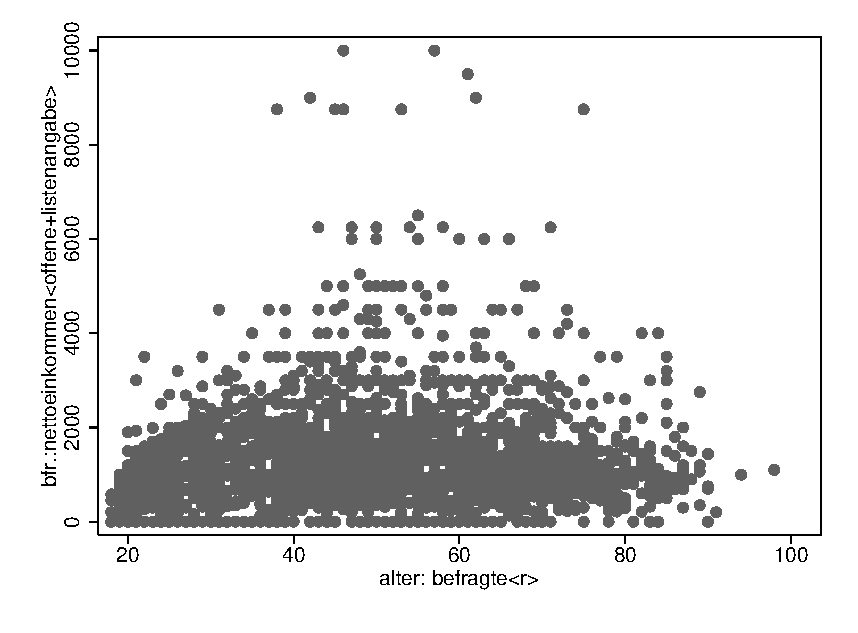
\includegraphics[width=8cm]{images/scatter.eps}}
\end{figure}
\end{frame}

\section{Boxplots}
\begin{frame}[fragile]{Boxplots} \index{Grafik!Boxplots} \index{Grafik!graph box}
\begin{lstlisting}
graph box hhinc
\end{lstlisting}
\begin{figure}
{\centering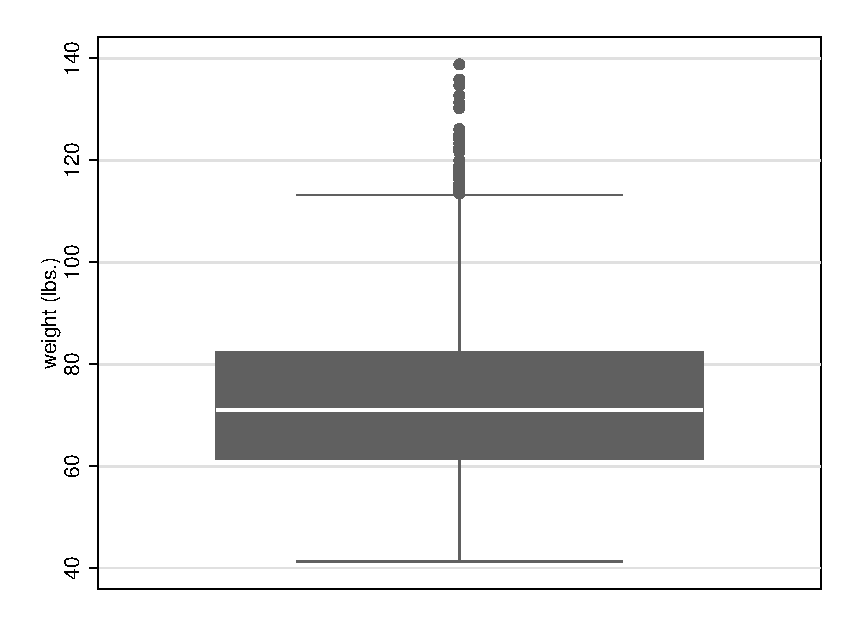
\includegraphics[width=8cm]{images/box.eps}}
\end{figure}
\end{frame}

\section{Histogramme}
\begin{frame}[fragile]{Histogramme} \index{Grafik!Histogramme} \index{Grafik!hist} \index{Grafik!hist freq}
\begin{lstlisting}
hist hhinc, freq
\end{lstlisting}
\begin{figure}
{\centering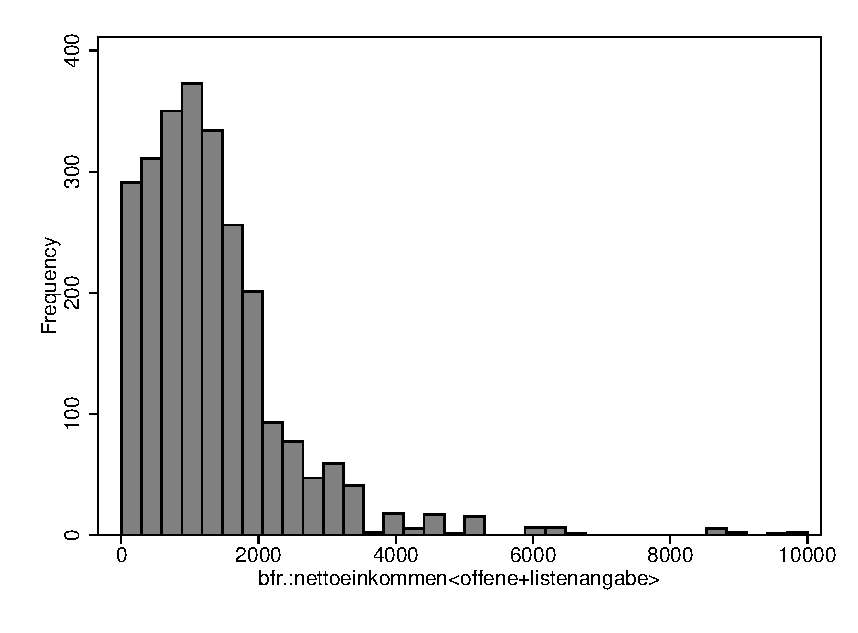
\includegraphics[width=8cm]{images/hist.eps}}
\end{figure}

  \begin{tikzpicture}[transform shape, rotate=10, overlay]
\node at (8,2) [mybox] (box) {%
    \begin{minipage}[t!]{0.35\textwidth}
    \tiny\textcolor{black}{\texttt{freq erzeugt Häufigkeiten, sonst steht auf der y-Achse die Dichte.}}
    \end{minipage}
    };
\end{tikzpicture}

\end{frame}

\section{Dot-Charts}
\begin{frame}[fragile]{Dot-Charts} \index{Grafik!Dot-Charts} \index{Grafik!graph dot} \index{Grafik! graph dot over()}
\begin{lstlisting}
graph dot (mean) hhinc, over(sex)
\end{lstlisting}
\begin{figure}
{\centering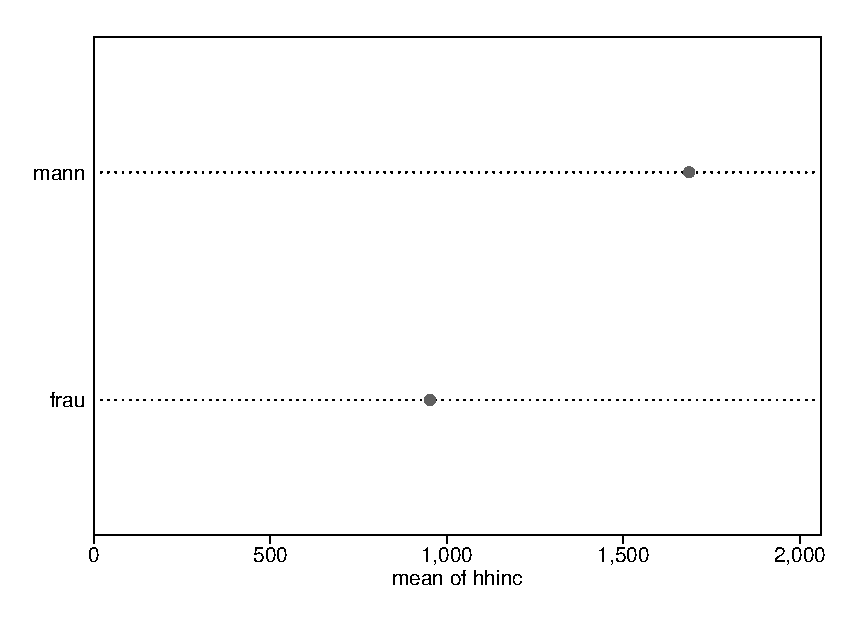
\includegraphics[width=8cm]{images/dot.eps}}
\end{figure}
\end{frame}


\section{Export von Grafiken}
\begin{frame}[fragile]{Export von Grafiken} \index{Grafik!exportieren}
\begin{lstlisting}
graph export "${OUTPUT}\graph1.pdf", replace
\end{lstlisting}
\begin{itemize}
\item Zum Export von Grafiken stehen mehrere Formate zur Verfügung
\item .ps .pes .wmf .emf .pdf .png .tif
\item Zur Weiterverarbeitung in MS-Office Programmen empfiehlt sich .png
\item Zur Weiterverarbeitung in TeX empfiehlt sich .pdf oder .eps
\end{itemize}
\end{frame}
%%%
%%% Improved Datahandling
%%%
\part{Improved Datahandling}
\begin{frame}
\thispagestyle{empty}
\textbf{\huge{Improved\\ Datahandling}}
\end{frame}

\begin{frame}{Improved\\ Datahandling Contents}
 \tableofcontents
\end{frame}

\section{by}
\begin{frame}[fragile]{by I} \index{by} \index{by!bysort}
Select subsets
\begin{lstlisting}
  summarize weight if sex == 1
  summarize weight if sex == 2
\end{lstlisting}

Do it in a single line
\begin{lstlisting}
  by edu, sort: summarize hhinc
\end{lstlisting}

  \begin{tikzpicture}[transform shape, rotate=10, overlay]
\node at (7.5,-0.5) [mybox] (box) {%
    \begin{minipage}[t!]{0.35\textwidth}
    \tiny\textcolor{black}{\texttt{by is not allowed with every command, in doubt contact the help. To use by cases have to be sorted. Alternativ: bysort}}
    \end{minipage}
    };
\end{tikzpicture}
\end{frame}

\begin{frame}[fragile]{by II}
Es können auch mehrere Variablen genommen werden \index{by}
\begin{lstlisting}
  by sex county, sort: summarize weight
\end{lstlisting}
\end{frame}

\section{in}
\begin{frame}[fragile]{in}
Select only a few cases \index{list}
\begin{lstlisting}
  ** select the first
  list sex in 1
  ** select the first ten
  list sex in 1/10
\end{lstlisting}

  \begin{tikzpicture}[transform shape, rotate=10, overlay]
\node at (7.5,-0.5) [mybox] (box) {%
    \begin{minipage}[t!]{0.35\textwidth}
    \tiny\textcolor{black}{\texttt{Usually single cases are not interesting, but this can be helpful to spot strange cases.}}
    \end{minipage}
    };
\end{tikzpicture}
\end{frame}


\section{Loops}
\begin{frame}[fragile]{Loops I} \index{Loops} \index{Loops!foreach}
Loops in Stata. Example from \textcite[69f.]{Kohler2012}
\begin{lstlisting}
** Generate variables r1 - r10
** Newlist
foreach var of newlist r1-r10 {
  gen `var' = runiform()
}

** Numeric list
foreach num of numlist 1/10 {
  replace r`num' = runiform()
}
\end{lstlisting}
\end{frame}

\begin{frame}[fragile]{Loops II} \index{Loops} \index{Loops!foreach} \index{Loops!forvalues}
\begin{lstlisting}
** multiple commands in a loop
foreach var of varlist ybirth income {
  summarize `var', meanonly
  generate `var'_c = `var' - r(mean)
  label variable `var'_c "`var' (centered)"
}
\end{lstlisting}

\begin{lstlisting}
** Forvalues
forvalues num = 1/10 {
  replace r`num' = runiform()
}
\end{lstlisting}
\end{frame}

\section{log-files}
\begin{frame}[fragile]{log-files} \index{log} \index{log!log-files}
  \begin{itemize}
    \item Results can be stored in log-files.
    \item These contain all commands and their results.
    \item Logging begins after
    \begin{lstlisting}
  log using <dateiname.log>
    \end{lstlisting}
    \item log-files can be opened with every texteditor.
  \end{itemize}
\end{frame}

\begin{frame}[fragile]{log-files II}
  \begin{itemize} \index{log} \index{log!using} \index{log!close}
   \item Define a name and path where the log-file is saved. Usually the log-file name should reflect the do-files name.
   \begin{lstlisting}
  log using read-soep.log, replace
   \end{lstlisting}
   \item At the end of the do-file
   \begin{lstlisting}
  ** commands will not be logged after this
  log close
   \end{lstlisting}
   \item Thrown errors stop the do-files execution, therefore a manual closing of the log-file might be required because Stata cannot handle two open log-files
   \begin{lstlisting}
  log close
   \end{lstlisting}
  \end{itemize}
  
    \begin{tikzpicture}[transform shape, rotate=10, overlay]
\node at (7.5,-0.5) [mybox] (box) {%
    \begin{minipage}[t!]{0.35\textwidth}
    \tiny\textcolor{black}{\texttt{capture log close atop log using ensures that all open log-files will be closed.}}
    \end{minipage}
    };
\end{tikzpicture}
\end{frame}

\section{Macros}
\begin{frame}[fragile]{Macros} \index{Macros} \index{Macros!global}
With longer pathes and bigger projects it is helpful to use so called Macros. Macros may be global (it is known everywhere inside your code) or local (it is known only in a specific loop). We use macros for paths
\begin{lstlisting}
  ** global Macroname Pathname
  global DATA "D:/Data/data/original/"
  global OUT "D:/Data/data/bearbeitet/"
\end{lstlisting}
Now the macros can be called like this
\begin{lstlisting}
 cd "${DATA}"
\end{lstlisting}

\end{frame}

\begin{frame}[fragile]{Macros II}
It is especially helpfull handling long or different directorys for input, output, images or log files. Some additional examples \index{Macros}
\begin{lstlisting}
  use "${DATA}testdata.dta", clear
  save "${OUT}testdata_recoded.dta", replace
\end{lstlisting}
The syntax readability benefits a lot from this

  \begin{tikzpicture}[transform shape, rotate=10, overlay]
\node at (7.5,-2.1) [mybox] (box) {%
    \begin{minipage}[t!]{0.35\textwidth}
    \tiny\textcolor{black}{\texttt{Your saving time. Long paths are written once, which minimizes typos. A correct macros is correct for the full document. Still macros don't help you with thinking.}}
    \end{minipage}
    };
\end{tikzpicture}

\end{frame}

\section{Using}
\begin{frame}[fragile]{using} \index{Import!use using} \index{Sort!sort}
Stata can handle only a limited range of variables, so a little housekeeping is advised.\footnote{Different Stata versions have different limits: IC (the version your working with) can handle $2,047$, SE can handle $32,767$ variables. Handling more variables is rather expensive. Prices for 2013: \$189 and \$395 for students. Non academic single user licenses \$$1545$ and \$$2090$.} Handling the SOEP this limit is not as far away as you might believe.
\begin{lstlisting}
  ** Import a minimal ppfad
  ** kepp only hhnr persnr sex gebjahr
  use hhnr persnr sex gebjahr using "${DATA}ppfad.dta"
  ** Sort cases by persnr and gebjahr
  sort persnr gebjahr
\end{lstlisting}
\end{frame}

\section{Merge}
\begin{frame}{merge} \index{Merge!merge}
\begin{minipage}{11cm}
In the Sozio-oekonomischen Panel (SOEP) (s. \cite{Wagner07}) each years data is split into different smaller data files. This has historical and maybe even practical reasons.\\
Starting from a file different of these data files share, we can combine the smaller files to generate a complete data set. This combination is called \textit{merging}.
\end{minipage}
\end{frame}

\begin{frame}[fragile]{merge II} \index{Merge!merge}
\begin{minipage}{11cm}
As example: We merge \textbf{ppfad} with \textbf{bep} and \textbf{bepgen}. \textbf{ppfad} is the data file ever person file shares. To make sure that we combine only persons data correct, we seek for matches of household-id (hhnr) and person-id (persnr).\\

\begin{tikzpicture}[thick]
\node at ( 3,2) [rectangle,draw=black,text width=4cm,align=center] (ppfad) {ppfad \\
									    hhnr, persnr};

\node at ( 0,0) [rectangle,draw=black,text width=4cm,align=center] (bekind) {bep \\
									    hhnr, persnr};
\node at ( 6,0) [rectangle,draw=black,text width=4cm,align=center] (bepgen) {bepgen \\
									    hhnr, persnr};
									    
\draw[->] (bekind) -- (ppfad);
\draw[->] (bepgen) -- (ppfad);
\end{tikzpicture}
\end{minipage}
\end{frame}


\begin{frame}[fragile]{merge III}
Running \texttt{merge} \index{Merge!merge}

\begin{lstlisting}
  ** merge ppfad with 2014 bep
  merge 1:1 persnr using "${DATA}bep.dta"
\end{lstlisting}

\begin{table}
\begin{center}
\begin{scriptsize}
\begin{tabular}{lll}
 Result & \# of obs. & \\ 
 \midrule
 not matched & 25,834 & \\
 ~~from master & 25,834  &(\_merge==1) \\
 ~~from using  & 0 &(\_merge==2) \\
 & & \\
 matched & 10,471 & (\_merge==3) \\
 \midrule
\end{tabular}
\end{scriptsize}
\end{center}
\end{table}
This means 
\begin{itemize}
 \item $25,834$ cases of \texttt{ppfad} were not found in \texttt{bep}.
 \item $0$ cases of \texttt{bep} were not found in \texttt{ppfad}
 \item $10,471$ cases of \texttt{bep} were found in \texttt{ppfad}
\end{itemize}
\end{frame}

\begin{frame}[fragile]{merge IV}\index{Merge!\_merge}\index{Merge!merge}
\begin{minipage}{11cm}
A new variable \texttt{\_merge} is created containing the \texttt{\_merge==} values. For now we remove all cases where we could not find a match from \texttt{using} which is \texttt{\_merge==2}. These are potentially problematic as we have no information about these persons sex or year of birth. Lucky at our current stage these are zero cases. Afterwards we remove \texttt{\_merge}.
\begin{lstlisting}
  ** Drop if using does not match master
  drop if _merge==2
  ** drop _merge
  drop _merge
\end{lstlisting}
\end{minipage}


  \begin{tikzpicture}[transform shape, rotate=10, overlay]
\node at (7.5,-1.5) [mybox] (box) {%
    \begin{minipage}[t!]{0.35\textwidth}
    \tiny\textcolor{black}{\texttt{The coice which merge is dropped is depending on the analysis.}}
    \end{minipage}
    };
\end{tikzpicture}

\end{frame}

\begin{frame}[fragile]{merge V} \index{Merge!merge} \index{Merge!merge, keepusing}
Example: merge with the generated variable highest educational achievement \texttt{bepsbil} from data-file \textbf{bepgen}.

\begin{lstlisting}
  merge 1:1 hhnr persnr using "${DATA}bepgen.dta", keepusing(bepsbil)
  drop if _merge==2
  drop _merge
\end{lstlisting}

  \begin{tikzpicture}[transform shape, rotate=10, overlay]
\node at (7.5,-1.5) [mybox] (box) {%
    \begin{minipage}[t!]{0.35\textwidth}
    \tiny\textcolor{black}{\texttt{In \textbf{bepgen} contains $65$ variables, but all we need is the educational achievement.}}
    \end{minipage}
    };
\end{tikzpicture}
\end{frame}

\section{Operators}
\begin{frame}[fragile]{Operators} \index{Operators}
Stata list the following operators, which can be used with variables. Using \texttt{var1\^{}2} every value of \texttt{var1} will be squared.
\begin{lstlisting}
 == // equals
 != // not equal ~=
 & // and
 | // or
 ! // not
 < // smaller
 > // greater
 <= // smaller equal
 >= // greater equal
 + // plus
 - // minus
 / // divide
 * // mutiply
 ^ // power
\end{lstlisting}
\end{frame}

\begin{frame}[fragile]{Functions} \index{Functions}
Additionaly Stata contains a range of built in functions (\texttt{help functions}).
A selection:
\begin{lstlisting}
  abs() // absolute value/modulus |-2| == 2
  max() // greates value
  min() // smalles value
  exp() // e-function
  ln() // logarithm
  round() // round
  sin() // Sinus
  sqrt() // square root
  runiform() // random number
\end{lstlisting}
\end{frame}
%%%
%%% Statistics
%%%
\part{Statistics}
\begin{frame}
\thispagestyle{empty}
\textbf{\huge{Statistics}}
\end{frame}

\begin{frame}{Statistics Contents}
 \tableofcontents
\end{frame}


\section{Statistic}
\begin{frame}[fragile]{Statistic I}
Arithmetic mean and some additional statistics \index{Mean!mean} \index{Describe!summarize} \index{Describe!detail} \index{Mean} \index{Statistic}
\begin{lstlisting}
  mean height
  summarize height
  summarize height, detail
\end{lstlisting}

  \begin{tikzpicture}[transform shape, rotate=10, overlay]
\node at (8,-1.5) [mybox] (box) {%
    \begin{minipage}[t!]{0.35\textwidth}
    \tiny\textcolor{black}{\texttt{mean returns the standard error: $s/\sqrt{n}$. summarize returns the standard deviation: $\sqrt{\sum(x-\bar{x})^2)/n}$.}}
    \end{minipage}
    };
\end{tikzpicture}
\end{frame}


\begin{frame}[fragile]{Statistic II}
Minimum, maximum, arithmetic mean, median, number of observations and quartils. \index{Minimum} \index{Minimum!min} \index{Maximum} \index{Maximum!max} \index{Mean!mean} \index{Mean} \index{Mean!arithmetic mean} \index{Mean!Median} \index{Quantile} \index{tabstat} \index{Range} \index{Range!range} \index{Quantile!q}
\begin{lstlisting}
  tabstat height, statistic(min max mean median p50)
  tabstat height, statistic(min max range mean count q) by(county)
\end{lstlisting}

  \begin{tikzpicture}[transform shape, rotate=10, overlay]
\node at (8,-1.5) [mybox] (box) {%
    \begin{minipage}[t!]{0.35\textwidth}
    \tiny\textcolor{black}{\texttt{range = max - min}}
    \end{minipage}
    };
\end{tikzpicture}
\end{frame}


\begin{frame}[fragile]{Maßzahlen III}
Standard deviation, standard error, variance und interquartil range. \index{Standard deviation} \index{Standard error} \index{Variance} \index{Interquartil range} \index{tabstat} \index{Standard deviation!sd} \index{Variance!var} \index{Standard error!sem} \index{Interquartil range!iqr} \index{Quantile!q} \index{Skewness} \index{Kurtosis} \index{Skewness!skewness} \index{Kurtosis!kurtosis}
\begin{lstlisting}
 tabstat height, statistic(sd sem var q iqr)
\end{lstlisting}
Skewness and kurtosis
\begin{lstlisting}
  tabstat height, statistics(skewness kurtosis)
\end{lstlisting}

  \begin{tikzpicture}[transform shape, rotate=10, overlay]
\node at (8,-1.5) [mybox] (box) {%
    \begin{minipage}[t!]{0.35\textwidth}
    \tiny\textcolor{black}{\texttt{iqr = q3 - q1}}
    \end{minipage}
    };
\end{tikzpicture}
\end{frame}

\section{Tables}
\begin{frame}[fragile]{Tables} \index{Table!tab} \index{Table!tab, summarize()} \index{Table}
We already had \texttt{summarize} and \texttt{tab}, let us combine them
\begin{lstlisting}
  tab county, summarize(height)
\end{lstlisting}
\end{frame}

\subsection{Cross tabs}
\begin{frame}[fragile]{Cross tabs} \index{Table!tab} \index{Table!tab1} \index{Table!tab2} \index{Table!cross tab}
Create a cross tab with
\begin{lstlisting}
  tab school county
\end{lstlisting}
And some more tables
\begin{lstlisting}
  ** tabs of each variable
  tab1 sex county school
  ** cross tabs of ab bc ac
  tab2 sex county school
\end{lstlisting}
\end{frame}

\subsection{Chi, V and Phi}
\begin{frame}[fragile]{Cross tabs II} \index{Table!cross tab} \index{Table!$\chi^2$} \index{Table!chi-square} \index{Table!chi} \index{Table!tab} \index{Table!Cramers V} \index{Table!tab exp} \index{Table!tab col} \index{Table!tab row}
Let us recapitulate Statistics I, we will do some tests \footnote{or see e.g. \textcite{Krebs10} oder \textcite{Agresti09}.}
\begin{lstlisting}
** chi^2
tab sex county, chi
** cramers v
tab sex county, V

** manual
tab sex county, exp col row
** phi and for 2x2 tabs V
di (1013*1002 - 925*1131) / (2144*1927*1938*2133)^(1/2) 
** chi^2
di 4071 *(-.00753735)^2
** usual way to compute V
di (.23128021 / 4071 * (2 - 1) )^(1/2) // V
\end{lstlisting}
\end{frame}

\begin{frame}[fragile]{Numlabel}
You can add numeric values to your variable labels \index{Label!numlabel}
\begin{lstlisting}
  ** numeric labels on for all variables
  numlabel _all, add
  ** and off
  numlabel _all, remove
\end{lstlisting}
\end{frame}

\section{Inference}
\begin{frame}[fragile]{T-Test} \index{T-Test!ttest} \index{T-Test}
And finally let us have a look at some test-statistics
\begin{lstlisting}
  ** compare 
  tab sex, sum(bmi)
  ttest bmi, by(sex)
\end{lstlisting}
\end{frame}

\begin{frame}[fragile]{And much more to come \dots} \index{Regression!regress} \index{Regression!logit} \index{Regression!mlog}
Regression
\begin{lstlisting}
  regress
  logit
  mlog
\end{lstlisting}
\end{frame}

\begin{frame}
\thispagestyle{empty}
 To be continued.
\end{frame}



\part{Index und Literatur}
\begin{frame}
\thispagestyle{empty}
\textbf{\huge{Index \\ and Literature}}
\end{frame}

\section{Index}
\begin{frame}{Index}
\setlength{\columnseprule}{.4pt} 
\begin{multicols}{5}
 \begin{miniscule}
  \printindex
 \end{miniscule}
\end{multicols}
\end{frame}

\section{Literature}
\begin{frame}[allowframebreaks]{Literature}
 \printbibliography[title=none]
\end{frame}

\end{document}
